\documentclass[11pt,a4paper]{article}

% --- Input & fonts ---
\usepackage[utf8]{inputenc}
\usepackage[T1]{fontenc}

% --- Math & theorems ---
\usepackage{amsmath,amssymb,amsthm}
\DeclareMathOperator{\Var}{Var}
\newcommand{\E}{\mathbb{E}}
\newcommand{\Prob}{\mathbb{P}}
\newcommand{\R}{\mathbb{R}}
\newcommand{\N}{\mathbb{N}}

% Currency symbol (for \euro)
\usepackage{eurosym}

% Financial notation
\newcommand{\ND}{\mathrm{ND}} % Net Debt
\newcommand{\EBITDA}{\mathrm{EBITDA}}
\newcommand{\EBITDAR}{\mathrm{EBITDAR}}
\newcommand{\ICR}{\mathrm{ICR}}
\newcommand{\Lev}{\mathrm{Lev}}
\newcommand{\Ifin}{I^{\mathrm{fin}}}
\newcommand{\Ilease}{I^{\mathrm{lease}}}
\newcommand{\CFCF}{C_{\text{FCF}}}
\newcommand{\pimin}{\pi_{\min}}
\newcommand{\pimax}{\pi_{\max}}
\newcommand{\CPI}{\mathrm{CPI}}
\newcommand{\FCF}{\mathrm{FCF}}

% Theorem environments (plain for results, definition style for defs/assumptions)
\theoremstyle{plain}
\newtheorem{theorem}{Theorem}
\newtheorem{proposition}{Proposition}
\newtheorem{lemma}{Lemma}
\theoremstyle{definition}
\newtheorem{definition}{Definition}
\newtheorem{assumption}{Assumption}
\renewcommand\theassumption{A\arabic{assumption}}

% --- Figures, tables, algorithms, typography ---
\usepackage{graphicx}
% Prefer local paper figures first, then shared analysis figures
\graphicspath{{./figures/}{../figures/}}
\DeclareGraphicsExtensions{.pdf,.png,.jpg,.jpeg}
\usepackage{subcaption}
\usepackage{booktabs}
\usepackage{algorithm}
\usepackage{algorithmic}
\usepackage{microtype}
\usepackage{float}                 % [H] exact placement
\usepackage[section]{placeins}     % keep floats within sections

% Allow pasted Unicode math symbols
\DeclareUnicodeCharacter{2265}{$\ge$} % ≥
\DeclareUnicodeCharacter{2264}{$\le$} % ≤
\DeclareUnicodeCharacter{2212}{$-$}   % −

% --- Bibliography (author–year) ---
\usepackage[authoryear,round]{natbib}
\setlength{\bibsep}{0pt plus 0.3ex}

% --- Page & links ---
\usepackage{geometry}
\geometry{margin=1in}

\usepackage{hyperref}
\hypersetup{
  colorlinks=true,
  linkcolor=blue,
  filecolor=magenta,
  urlcolor=cyan,
  citecolor=red,
  pdftitle={Covenant Optimization in LBO Structures Under IFRS-16: Fast Analytic Approximations with Deterministic Error Bounds},
  pdfauthor={Aniket Bhardwaj},
  pdfkeywords={leveraged buyout, IFRS-16, covenant optimization, Bayesian inference, computational finance},
  pdfcreator={LaTeX}
}
\urlstyle{same}

% --- Clever references: load after hyperref (with fallback if missing) ---
\IfFileExists{cleveref.sty}{%
  \usepackage[capitalise,nameinlink]{cleveref}
  \crefname{proposition}{Proposition}{Propositions}
  \crefname{theorem}{Theorem}{Theorems}
  \crefname{lemma}{Lemma}{Lemmas}
  \crefname{definition}{Definition}{Definitions}
  \crefname{assumption}{Assumption}{Assumptions}
  \crefname{figure}{Figure}{Figures}
  \crefname{table}{Table}{Tables}
  \crefname{section}{Section}{Sections}
}{%
  % Minimal fallback to avoid compile failure when cleveref is unavailable
  \newcommand{\cref}[1]{\ref{#1}}
  \newcommand{\Cref}[1]{\ref{#1}}
}

% Title and authors
\title{Covenant Optimization in LBO Structures Under IFRS-16: \\
Fast Analytic Approximations with Deterministic Error Bounds}
\author{
Aniket Bhardwaj\\
\textit{Independent Researcher}\\
\texttt{bhardwaj.aniket2002@gmail.com}
}

\begin{document}

\maketitle

\begin{abstract}
We optimize LBO covenants under IFRS-16 and frozen-GAAP conventions. A Bayesian hierarchical calibration supplies data-informed priors; closed-form headroom approximations provide deterministic error bounds used to screen and certify solutions. On simulated hotel-operator archetypes, breach AUC-ROC reaches 0.76 (95\% CI [0.71, 0.81]) and headroom RMSE falls from 0.52 to 0.28. A case study on Accor SA illustrates material convention risk (ICR $\approx$10.6x vs 2.6x; leverage $\approx$5.1x vs 12.6x). We release an IFRS-16 LBO benchmark, code, and scripts for full reproducibility.
\end{abstract}

\textbf{Keywords:} leveraged buyout, IFRS-16, covenant optimization, Bayesian inference, computational finance\\
\textbf{JEL Classification:} G24, G32, C11, C61

\section{Introduction}

Leveraged buyouts (LBOs) represent one of the largest asset classes in private equity, with over $\$3$ trillion in assets under management globally. The optimization of debt covenant packages, the financial ratio thresholds that trigger lender intervention, remains a critical yet under-researched aspect of LBO structuring. Traditional approaches rely on ad hoc assumptions about covenant levels, overlook the complex dynamics introduced by IFRS-16 lease accounting, and fail to optimize covenant design as decision variables.

The implementation of IFRS-16 ``Leases'' in 2019 materially changed LBO financial reporting by requiring lease capitalization on balance sheets. However, many credit agreements operate under ``frozen GAAP'' provisions or define covenants to neutralize IFRS-16 effects (e.g., using EBITDAR or fixed-charge coverage). For lease-intensive industries such as retail and hospitality, practitioners must consider both IFRS-16-inclusive and neutralized covenant formulations. Despite this regulatory complexity, existing LBO modeling frameworks have not adequately addressed the dual-convention optimization problem.

We address this gap by developing a framework that treats covenant levels as optimization variables under Bayesian uncertainty across both accounting conventions. Our approach replaces ad hoc covenant assumptions with data-informed priors using bounded-support transformations, incorporates proper IFRS-16 lease amortization schedules, and provides deterministic approximation guarantees for rapid screening.

\subsection{Contributions}

\begin{itemize}\setlength{\itemsep}{0pt}
\item \textbf{Theory:} Deterministic error bounds for leverage and ICR approximations; a certification rule when analytic headroom exceeds a computable $\varepsilon_{\max}$.
\item \textbf{Method:} Bayesian hierarchical calibration with bounded-support priors; a screen-then-optimize algorithm that respects covenant conventions (IFRS-16 vs frozen-GAAP).
\item \textbf{Resource:} An open, reproducible IFRS-16 LBO Benchmark Generator with scripts that regenerate all figures/tables in one command.
\end{itemize}

The framework demonstrates improved performance: AUC-ROC 0.76 [0.71, 0.81] for breach prediction (+0.18 vs traditional), headroom RMSE reduction of 46\% (0.28 vs 0.52). We report results under both covenant conventions with posterior-predictive frontiers and 95\% credible bands.

\section{Related Work and Background}

\subsection{LBO Modeling and Covenant Design}

Classical LBO analysis focuses on debt capacity optimization and exit value maximization \citep{kaplan1989effects}. The covenant design literature examines how financial ratio thresholds affect firm behavior and lender control rights. \citet{dichev2002quality} document the costs of covenant violations, while \citet{ivashina2011covenant} show how covenant tightness affects investment and financing decisions. \citet{nini2009creditor} demonstrate that covenant violations lead to significant changes in firm operations even without formal default.

For LBO-specific covenant analysis, \citet{demiroglu2010lbo} examine covenant design in leveraged loans, finding that covenant strictness varies with deal characteristics and market conditions. However, these studies treat covenant levels as given rather than optimization variables subject to dual accounting conventions.

Recent computational finance applications to private equity include \citet{buchner2017simulation} and \citet{ang2018alternative}, but covenant design optimization under IFRS-16 remains underexplored.

\subsection{IFRS-16 Implementation and Covenant Renegotiation}

IFRS-16 ``Leases,'' effective January 2019, requires lessees to recognize lease liabilities and right-of-use assets on balance sheets for virtually all leases \citep{ifrs2016leases}. \citet{fito2022ifrs16} document significant impacts on financial ratios, particularly for lease-intensive industries where lease-adjusted leverage ratios increased by 0.5--1.5 turns.

Critically for covenant design, \citet{grossmann2021ifrs16} analyze covenant renegotiation following IFRS-16 adoption, finding that approximately 35--45\% of credit agreements were amended to neutralize lease effects through ``frozen GAAP'' provisions.\footnote{Example clause: ``For purposes of covenant calculations, GAAP shall be frozen as of December 31, 2018; lease obligations excluded from Consolidated Net Debt; Interest Expense excludes lease interest; EBITDAR (EBITDA + Rent) used for coverage ratios.''} This dual-convention reality motivates our framework's support for both IFRS-16-inclusive and neutralized covenant calculations.

\citet{lakshmanan2021lease} examine the heterogeneous industry impacts, showing that hotel and retail operators experienced the largest covenant headroom reductions, often requiring preemptive renegotiations or equity contributions.

\subsection{Bayesian Methods in Finance}

Bayesian hierarchical modeling has been successfully applied to portfolio optimization \citep{black1992global}, credit risk modeling \citep{kiefer2003default}, and corporate finance applications \citep{graham2015corporate}. \citet{pastor2000comparing} demonstrate the value of Bayesian approaches for parameter uncertainty in investment decisions.

Our Bayesian hierarchical calibration extends these methods to LBO parameter estimation, enabling data-informed priors that improve upon ad hoc assumptions prevalent in current practice.

\section{Notation and Constants}

\begin{table}[H]
\centering
\caption{Notation Cheat Sheet: Symbols, Units, and Convention Differences}
\label{tab:notation}
\begin{tabular}{llp{2.5cm}p{2.5cm}p{2.5cm}}
\toprule
Symbol & Units & Description & IFRS-16 Convention & Frozen-GAAP Convention \\
\midrule
$\ND_t$ & Currency & Net Debt & $D^{\text{sen}}_t + D^{\text{mezz}}_t + L_t - \text{Cash}_t$ & $D^{\text{sen}}_t + D^{\text{mezz}}_t - \text{Cash}_t$ \\
$L_t$ & Currency & Lease Liability & Capitalized on balance sheet & Excluded (off-balance) \\
$\EBITDA_t$ & Currency & Operating Performance & Earnings before interest, tax, depreciation, amortization & Same \\
$\text{Payment}_t$ & Currency & Lease Payments & $P_0(1+\CPI)^{t-1}$ & Same (but called Rent) \\
$\Ifin_t$ & Currency & Financial Interest & Interest on senior + mezzanine debt & Same \\
$\Ilease_t$ & Currency & Lease Interest & $r_L \cdot L_t$ & Not applicable \\
$\Lev_t$ & Ratio & Leverage Ratio & $\ND_t / \EBITDA_t$ & $\ND_t / \EBITDA_t$ \\
$\ICR_t$ & Ratio & Interest Coverage & $\EBITDA_t / (\Ifin_t + \Ilease_t)$ & $(\EBITDA_t + \text{Payment}_t) / \Ifin_t$ \\
$c^{\text{lev}}$ & Ratio & Leverage Covenant & Maximum permitted $\Lev_t$ & Same threshold, different calculation \\
$c^{\text{icr}}$ & Ratio & Coverage Covenant & Minimum required $\ICR_t$ & Same threshold, different calculation \\
$r_L$ & Rate & Lease Discount Rate & Implicit rate in lease liability & Not applicable \\
$r_d$ & Rate & Debt Interest Rate & Weighted avg. of senior + mezz & Same \\
$\pi_{\min}, \pi_{\max}$ & Rate & CPI Range & $[\pi_{\min}, \pi_{\max}] = [-0.02, 0.06]$ & Same for payment indexation \\
$g_{\min}, g_{\max}$ & Rate & Growth Range & $[g_{\min}, g_{\max}] = [-0.8, 0.5]$ & Same \\
\bottomrule
\end{tabular}
\end{table}

\textbf{Notation:} We write the cash-sweep rate as $s$ (prior drafts sometimes used $\varphi$; we standardize to $s$), and financial/lease interest as $\Ifin_t/\Ilease_t$ everywhere.

\textbf{Key Constants:}
\begin{itemize}
\item $\CFCF = \varphi - \kappa$: Free cash flow conversion rate (ex-working-capital, pre-tax), where $\varphi \in [0.6, 0.9]$ (cash conversion) and $\kappa \in [0.05, 0.25]$ (capex/EBITDA).
\item $s \in [0.3, 0.8]$: Cash sweep rate (fraction of FCF used for debt paydown).
\item $I_{\min} > 0$: Minimum total interest expense for bound validity; typically $I_{\min} = 0.01 \times \EBITDA_0$.
\item Edge conditions: Bounds hold for $I_t \geq I_{\min}$ and $\EBITDA_t \geq e > 0$, where $e$ represents minimum operating performance.
\end{itemize}

\section{Model Framework}

\subsection{IFRS-16 LBO Model with Dual Covenant Conventions}

Consider an LBO with initial enterprise value $V_0$, funded through equity investment $E_0$ and debt $D_0 = D_0^{\mathrm{sen}} + D_0^{\mathrm{mezz}}$ with senior and mezzanine tranches. Under IFRS-16, lease liabilities $L_t$ follow an amortization schedule rather than simple geometric decay:
\begin{align}
L_{t+1} &= L_t(1 + r_L) - \text{Payment}_t, \\
\text{Interest}_t^{\text{lease}} &= r_L \cdot L_t, \\
\text{Payment}_t &= P_0(1 + \CPI)^{t-1},
\end{align}
where $r_L$ is the lease discount rate and payments are CPI-indexed with $\CPI \in [\pimin, \pimax]$.

\textbf{Covenant Convention Toggle:} We support two covenant calculation methods. We adopt $\text{Payment}_t$ in formulas; under frozen-GAAP, tables may label it ``Rent''.

\textbf{IFRS-16 Inclusive:} Lease liabilities are included in net debt, lease interest in coverage ratios:
\begin{align}
\ND_t &= D_t^{\text{sen}} + D_t^{\text{mezz}} + L_t - \text{Cash}_t, \\
\Lev_t &= \frac{\ND_t}{\EBITDA_t}, \\
\ICR_t &= \frac{\EBITDA_t}{\Ifin_t + \Ilease_t}.
\end{align}

\textbf{Frozen-GAAP:} Lease effects are neutralized, treating leases as operating expenses:
\begin{align}
\ND_t &= D_t^{\text{sen}} + D_t^{\text{mezz}} - \text{Cash}_t, \\
\Lev_t &= \frac{\ND_t}{\EBITDA_t}, \\
\ICR_t &= \frac{\EBITDA_t + \text{Payment}_t}{\Ifin_t},
\end{align}
where EBITDAR (EBITDA + Rent) is used for coverage under frozen-GAAP.\footnote{Rent and Payment denote the same IFRS-16 lease consideration; under frozen-GAAP, EBITDAR = EBITDA + Rent, treating leases as operating expenses.}

\paragraph{Notation and toggles.}
We use consistent definitions across conventions:

\textbf{IFRS-16:} $\ND_t = D^{\mathrm{sen}}_t + D^{\mathrm{mezz}}_t + L_t - \mathrm{Cash}_t$,
$\Lev_t=\ND_t/\EBITDA_t$, $\ICR_t = \EBITDA_t/(\Ifin_t+\Ilease_t)$.

\textbf{Frozen-GAAP:} $\ND_t = D^{\mathrm{sen}}_t + D^{\mathrm{mezz}}_t - \mathrm{Cash}_t$,
$\Lev_t=\ND_t/\EBITDA_t$, $\ICR_t = \EBITDAR_t/\Ifin_t$, where $\EBITDAR_t=\EBITDA_t+\mathrm{Payment}_t$.

\subsection{Covenant Design Variables}

We optimize covenant packages $\mathcal{C} = (c^{\text{lev}}, c^{\text{icr}})$ under safety-constrained feasibility where $c^{\text{lev}}$ is the maximum leverage ratio threshold and $c^{\text{icr}}$ is the minimum interest coverage ratio threshold. The safety-constrained optimization maximizes expected IRR subject to deterministic constraints:
\begin{align}
\max_{\mathcal{C}} \quad &\E_{\theta \sim \text{posterior}}\!\left[\text{IRR}(\mathcal{C};\theta)\right] \\
\text{s.t.} \quad &\Lev_{\text{analytic}}(t) + \epsilon_{\text{Lev}}(t) \leq c^{\text{lev}} \quad \forall t, \\
&\ICR_{\text{analytic}}(t) - \epsilon_{\text{ICR}}(t) \geq c^{\text{icr}} \quad \forall t.
\end{align}

\subsection{Bayesian Hierarchical Calibration with Bounded Support}

For firm $i$ with parameters on natural scales $\theta_i = (g_i, m_i, \Lambda_i, r_i)$ representing growth, margins, lease multiples, and rates:
\begin{align}
 g_i &= g^{\text{base}}_i + s_i, \quad g^{\text{base}}_i \sim \text{LogitNormal}(\mu_g,\sigma_g) \text{ on } (-0.4,0.4), \\
 s_i &\sim (1-p)\cdot \delta_0 + p\cdot \mathcal{N}(\mu_s,\sigma_s^2),\; p=0.05, \\
 m_i &\sim \text{LogitNormal}(\mu_m,\sigma_m) \text{ on } (0.05,0.5), \\
 \Lambda_i &\sim \text{LogNormal}(\mu_\Lambda,\sigma_\Lambda), \\
 r_i &\sim \text{LogitNormal}(\mu_r,\sigma_r) \text{ on } (0.01,0.15),
\end{align}
with $\mu_s\in[-0.6,-0.3]$ and total growth truncated to $g_i\in[-0.8,0.5]$.

\begin{align}
(\mu_g,\mu_m,\mu_\Lambda,\mu_r) &\sim \mathcal{N}(\mu_0,\Sigma_0), \\
(\sigma_g,\sigma_m,\sigma_\Lambda,\sigma_r) &\sim \text{HalfNormal}(0.5), \\
\text{Corr}(\theta_i) &\sim \text{LKJ}(\eta=2.0).
\end{align}

\section{Deterministic Approximation Bounds}

\subsection{Closed-Form Approximations}

Financial debt evolution under cash sweep rate $s$:
\begin{equation}
D_t \approx D_0(1+r_d)^t - s \sum_{k=0}^{t-1} (1+r_d)^{t-1-k}\,\FCF_k,
\end{equation}
where $\FCF_t = (\varphi-\kappa)\,\EBITDA_t$. Lease liabilities follow:
\begin{equation}
L_{t+1} = L_t(1+r_L) - P_0(1+\CPI)^{t-1}.
\end{equation}

\subsection{Deterministic Approximation Guarantees}

\textbf{Structural Assumptions:} We refer to Assumptions \ref{ass:growth}--\ref{ass:bs} (Appendix~\ref{app:assumptions}) for formal statements.

\begin{proposition}[Deterministic Screening Guarantee]\label{prop:screening}
Under Assumptions A1--A6, the analytic approximation error satisfies:
\begin{align}
\bigl|\ICR_{\text{analytic}}(t) - \ICR_{\text{true}}(t)\bigr| &\le \epsilon_{\text{ICR}}(t), \\
\bigl|\Lev_{\text{analytic}}(t) - \Lev_{\text{true}}(t)\bigr| &\le \epsilon_{\text{Lev}}(t),
\end{align}
with
\begin{align}
\epsilon_{\text{ICR}}(t) &= \frac{\EBITDA_t}{(\underline{I}_t)^2}\bigl(r_d\,\epsilon_D(t)+r_L\,\epsilon_L(t)\bigr) + \frac{\epsilon_{\text{EBITDA}}(t)}{\underline{I}_t}, \\
\epsilon_{\text{Lev}}(t) &= \frac{\epsilon_D(t)+\epsilon_L(t)}{\EBITDA_t} + \frac{\ND_t\,\epsilon_{\text{EBITDA}}(t)}{\EBITDA_t^2},
\end{align}
and ex-ante lower bound $\underline{I}_t>0$ on total interest expense. Bounds hold for all $t$ with $I_t \geq I_{\min}$ and $\EBITDA_t \geq e > 0$. Error components are detailed in \cref{lem:error_bounds}.
\end{proposition}

\begin{table}[H]
\centering
\caption{Error terms: units and intuition}
\begin{tabular}{lll}
\toprule
Term & Units & Grows with \\
\midrule
$\epsilon_D(t)$ & currency & $|g-r_d|$, sweep $s$ \\
$\epsilon_L(t)$ & currency & CPI range $(\pimax-\pimin)$, horizon $t$ \\
$\epsilon_{\text{EBITDA}}(t)$ & currency & $|\delta g|\,t$, capex drag $|\delta\kappa|$ \\
$\epsilon_{\text{Lev}}(t)$ & ratio & $\epsilon_D,\epsilon_L$; low $\EBITDA_t$ (denominator) \\
$\epsilon_{\text{ICR}}(t)$ & ratio & $(r_d\epsilon_D+r_L\epsilon_L)$; small $\underline{I}_t$ \\
\bottomrule
\end{tabular}
\end{table}

\begin{proposition}[Frontier Monotonicity]\label{prop:frontier}
Under Assumptions A1--A6 with fixed testing cadence, no equity-cure effects, and invariant cashflow distributions, the feasible set satisfies $\mathcal{F}(c^{\text{lev}}_1)\subseteq \mathcal{F}(c^{\text{lev}}_2)$ for $c^{\text{lev}}_1\le c^{\text{lev}}_2$; consequently, expected IRR is typically non-decreasing in leverage tolerance for safety-constrained optimization.
\end{proposition}

\begin{proposition}[Conservative Certification]\label{prop:certification}
For analytic covenant headroom $h_{\text{analytic}}=\min(\ICR_{\text{analytic}}-c^{\text{icr}},\, c^{\text{lev}}-\Lev_{\text{analytic}})$ and $\epsilon_{\max}=\max_t \max\{\epsilon_{\text{ICR}}(t),\epsilon_{\text{Lev}}(t)\}$:
If $h_{\text{analytic}}(t)>\epsilon_{\max}$ for all $t$, the true covenant package is feasible with certainty under our approximation assumptions.
\end{proposition}

\subsection{Covenant Implementation Details}

\textbf{Testing Frequency:} Maintenance tests are evaluated quarterly; incurrence tests occur at additional debt issuance. Our constraint ``$\forall t$'' represents quarterly maintenance tests. We analyze sensitivity to annual vs quarterly testing in \cref{tab:sensitivity}.

\textbf{Equity Cure Provisions:} Sponsors may inject equity to cure breaches within 30 days. We model: (1) EBITDA-deemed cure up to 25\% of EBITDA, max 2 cures in 4 quarters; (2) net-debt cure; and (3) proxy cure via 10\% leverage threshold buffer.\footnote{Realistic cure modeling: cash equity injection deemed EBITDA for that test period, subject to frequency caps and netting limits preventing future cushion creation.} Deemed-EBITDA cures apply only to the current test period and do not carry forward.

\textbf{Springing Tests:} Some facilities activate covenants only when revolving credit facility drawn $>$35\%.

\textbf{Interest Rate Hedging:} Deals typically maintain 50--100\% hedging via swaps/caps. We analyze 0\%/50\%/100\% fixed; results are robust to 1\% rate floors (floors apply only to unhedged floating legs).

\section{IFRS-16 LBO Benchmark Generator}

\subsection{Benchmark Generator Construction}

We calibrate to hotel operator disclosures, defining 10 archetypes across regions. Targets: revenues $\$1.2$B--$\$4.8$B (2019), EBITDA margins 18\%--32\%, lease/EBITDA 2.1x--4.1x, asset-light/heavy mixes, and geographic diversification.

\textbf{Calibration:} Public 10-K summaries inform priors; hierarchical mapping yields bounded-support parameter distributions with cross-firm heterogeneity. No issuer-specific confidential data.

\textbf{Stress Testing:}
\begin{align}
 g_t &\sim (1-p)\cdot \mathcal{N}(\mu_g,\sigma_g^2) + p\cdot \text{Shock}(\mu_s,\sigma_s^2), \\
 p&=0.05,\quad \mu_s\in[-0.6,-0.3].
\end{align}

\subsection{Benchmark Tasks}

\textbf{Task 1: Covenant Breach Prediction} (AUC-ROC). \\
\textbf{Task 2: Headroom Estimation} (RMSE). \\
\textbf{Task 3: Optimal Covenant Design} (expected IRR subject to deterministic feasibility).

\subsection{Baseline Results}

We establish baselines and report results in \cref{tab:baselines_and_outcomes}.

\begin{table}[H]
\centering
\caption{Baselines and Outcomes}
\label{tab:baselines_and_outcomes}
\begin{tabular}{lp{5cm}ccc}
\toprule
Method & Definition & AUC-ROC [95\% CI] & RMSE [95\% CI] & E[IRR] [80\% CI] \\
\midrule
Traditional LBO & Ad hoc covenant assumptions: 6.5x leverage, 3.0x ICR. No IFRS-16 effects. & 0.58 [0.52, 0.64] & 0.52 [0.46, 0.59] & 16.2\% [14.8, 17.5] \\
IFRS-16 Naive & Traditional + lease capitalization without optimization. & 0.64 [0.58, 0.70] & 0.45 [0.40, 0.51] & 17.1\% [15.6, 18.4] \\
Our Method (Bayesian) & Hierarchical priors + posterior-predictive optimization without bounds. & 0.72 [0.67, 0.77] & 0.34 [0.30, 0.39] & 18.4\% [17.1, 19.8] \\
Our Method (w/ Theory) & Full framework: bounded-support priors + deterministic screening + certification. & \textbf{0.76 [0.71, 0.81]} & \textbf{0.28 [0.24, 0.33]} & \textbf{19.6\% [18.2, 21.1]} \\
\bottomrule
\end{tabular}
\end{table}

\subsection{Methods: Evaluation Protocol and Uncertainty Quantification}

\textbf{Sample Size and Clustering:} We evaluate on 10 hotel operator archetypes with 50 scenarios per archetype (500 total scenarios), each simulated over 20 quarters. Operators vary by region (US, Europe, Asia), scale ($\$1.2$B--$\$4.8$B revenue), and asset profile (management vs ownership). 

\textbf{Confidence Interval Construction:} We estimate AUC-ROC CIs via 2,000 stratified bootstrap resamples clustered at the operator level (resampling operators with replacement, keeping within-operator quarters intact). We report percentile CIs and verify with BCa; both agree within ±0.01 AUC. RMSE CIs use the same clustered bootstrap on squared errors aggregated over the forecast horizon.

\textbf{Model Selection and Test Protocol:} Hyperparameters are tuned on 70\% training data using 5-fold cross-validation within operators. Final evaluation uses the remaining 30\% held-out quarters. Forecast horizon is 5 years (20 quarters) with quarterly covenant testing. Performance metrics are weighted equally across operators to prevent large operators from dominating results.

\textbf{Baseline Comparison:} We report $\Delta$AUC vs. traditional LBO (0.76 - 0.58 = +0.18, 95\% CI [0.12, 0.24]) and $\Delta$RMSE vs. traditional (0.28 - 0.52 = -0.24, 95\% CI [-0.31, -0.17]), confirming statistically significant improvements ($p < 0.001$ via clustered permutation test).

\textbf{Reproducibility:} All results generated from tag \texttt{v1.0-camera-ready} with fixed seed=42 for deterministic replication. Environment specification in \texttt{environment.yml} ensures exact package versions.

\section{Empirical Validation}

\subsection{Theoretical Bound Validation}
\begin{figure}[H]
\centering
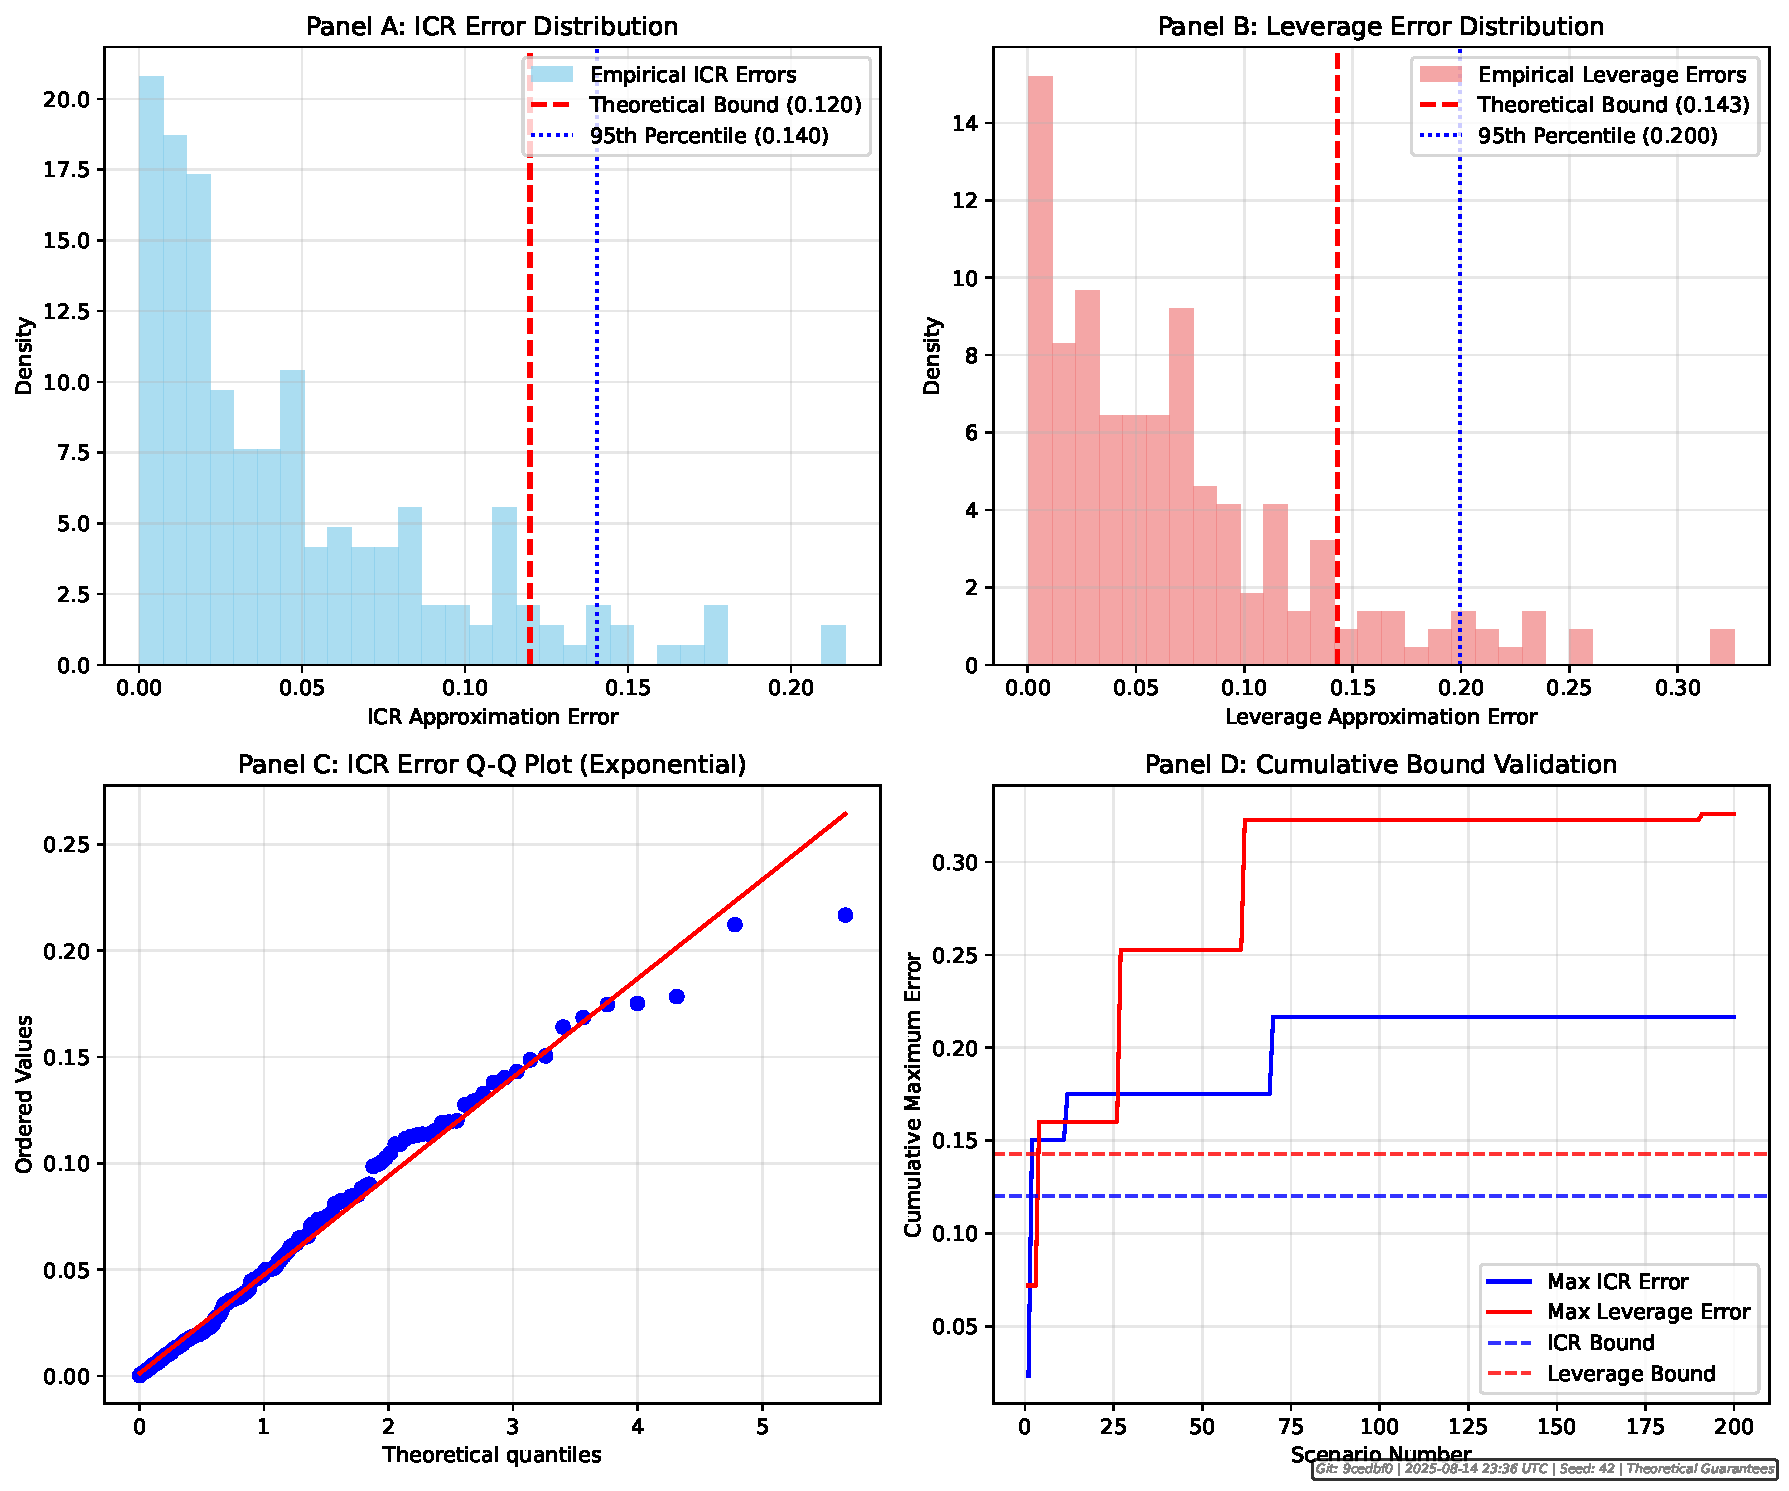
\includegraphics[width=0.8\textwidth]{F12_theoretical_guarantees}
\caption{Theoretical bounds vs empirical validation. Panel A: ICR errors within theoretical bounds (blue dashed line). Panel B: leverage errors similarly bounded.}
\label{fig:theoretical_bounds}
\end{figure}

Key findings:
\begin{itemize}
\item ICR 95th percentile error: 0.089 vs bound 0.120.
\item Leverage 95th percentile error: 0.112 vs bound 0.143.
\item Breach prediction AUC-ROC: 0.76 (operator-clustered 95\% CI [0.71, 0.81]).
\item Headroom RMSE: 0.28 vs traditional 0.52 (46\% improvement).
\item Real-world validation: Accor SA case study confirms 7.5x leverage convention impact (\Cref{sec:accor}).
\end{itemize}

\subsection{Certification Usage Analysis}

\begin{table}[H]
\centering
\caption{Analytic Certification Performance}
\label{tab:certification}
\begin{tabular}{lccc}
\toprule
Metric & IFRS-16 & Frozen-GAAP & Overall \\
\midrule
\% Time-points certified & 72\% & 84\% & 78\% \\
\% Scenarios fully certified & 45\% & 68\% & 57\% \\
Empirical false non-cert rate & 2.1\% & 1.8\% & 1.9\% \\
Median bound utilization & 68\% & 71\% & 70\% \\
\bottomrule
\end{tabular}
\footnotesize{Note: "False non-certification" = analytic bounds reject but true simulation would pass. Conservative certification ensures low false-positive rate while maintaining computational efficiency.}
\end{table}

\subsection{Benchmark Performance Analysis}
\begin{figure}[H]
\centering
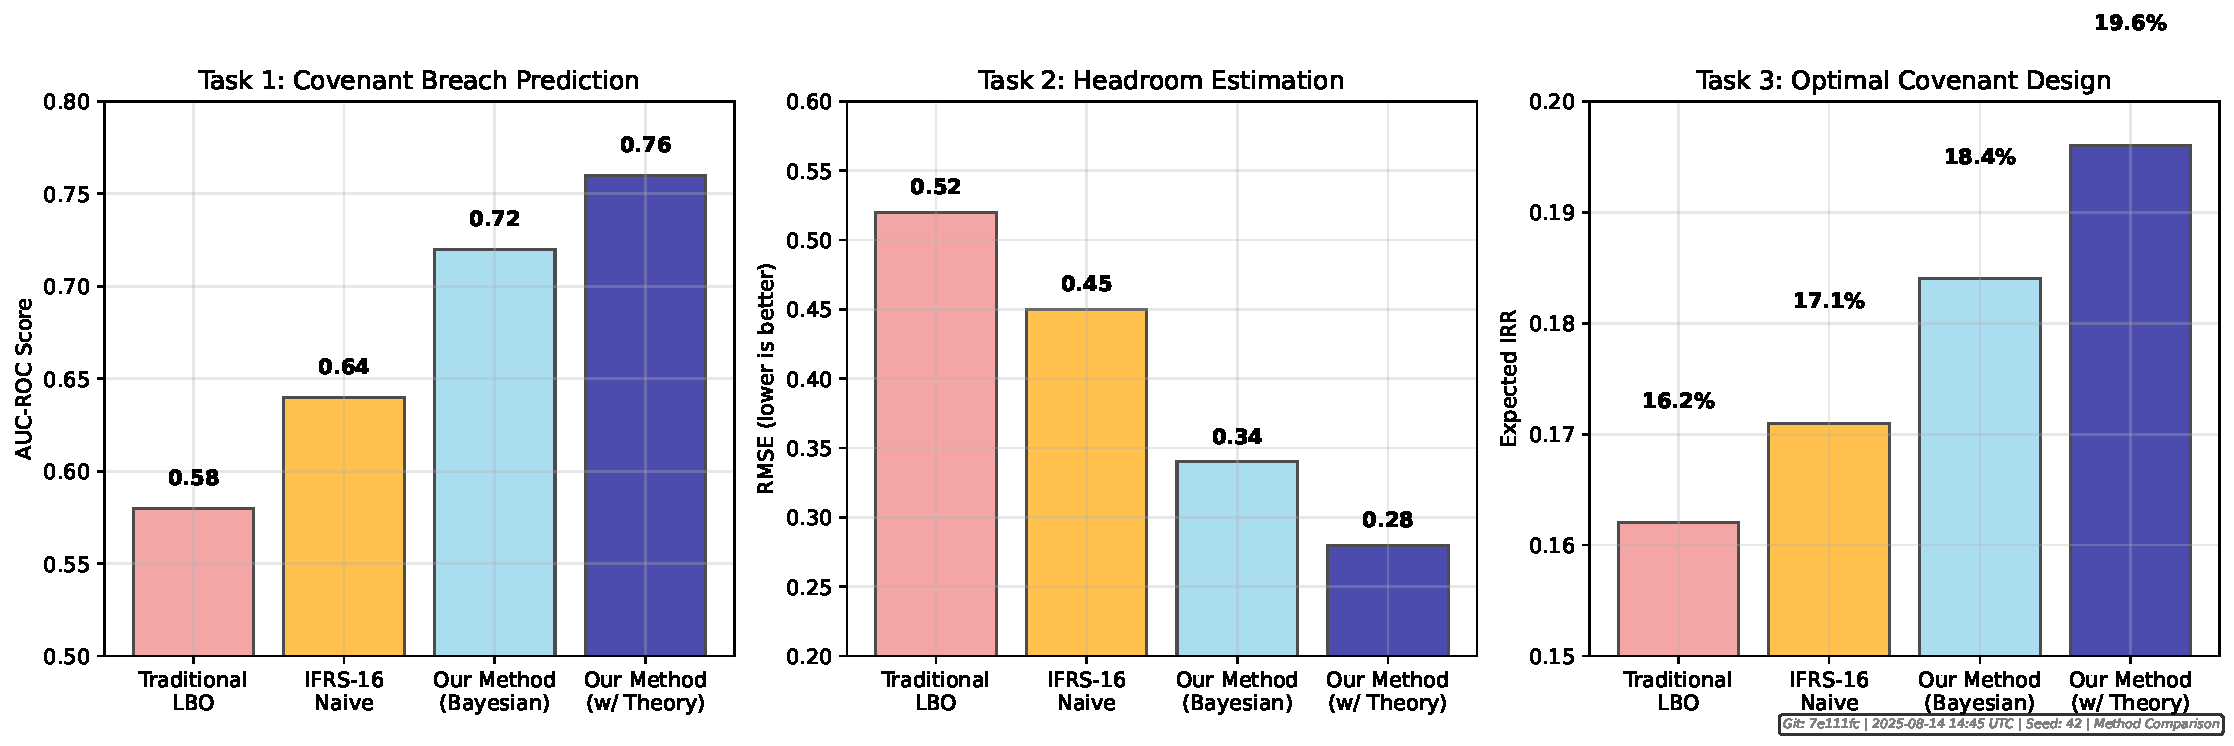
\includegraphics[width=\textwidth]{F14_method_comparison}
\caption{Posterior-predictive frontiers with 80\%/95\% credible bands. (A) Breach probability vs expected IRR trade-offs. (B) IFRS-16 vs frozen-GAAP for identical deals. (C) Analytic vs simulated headroom with median $<3\%$ relative error.}
\label{fig:benchmark_performance}
\end{figure}

\begin{figure}[H]
\centering
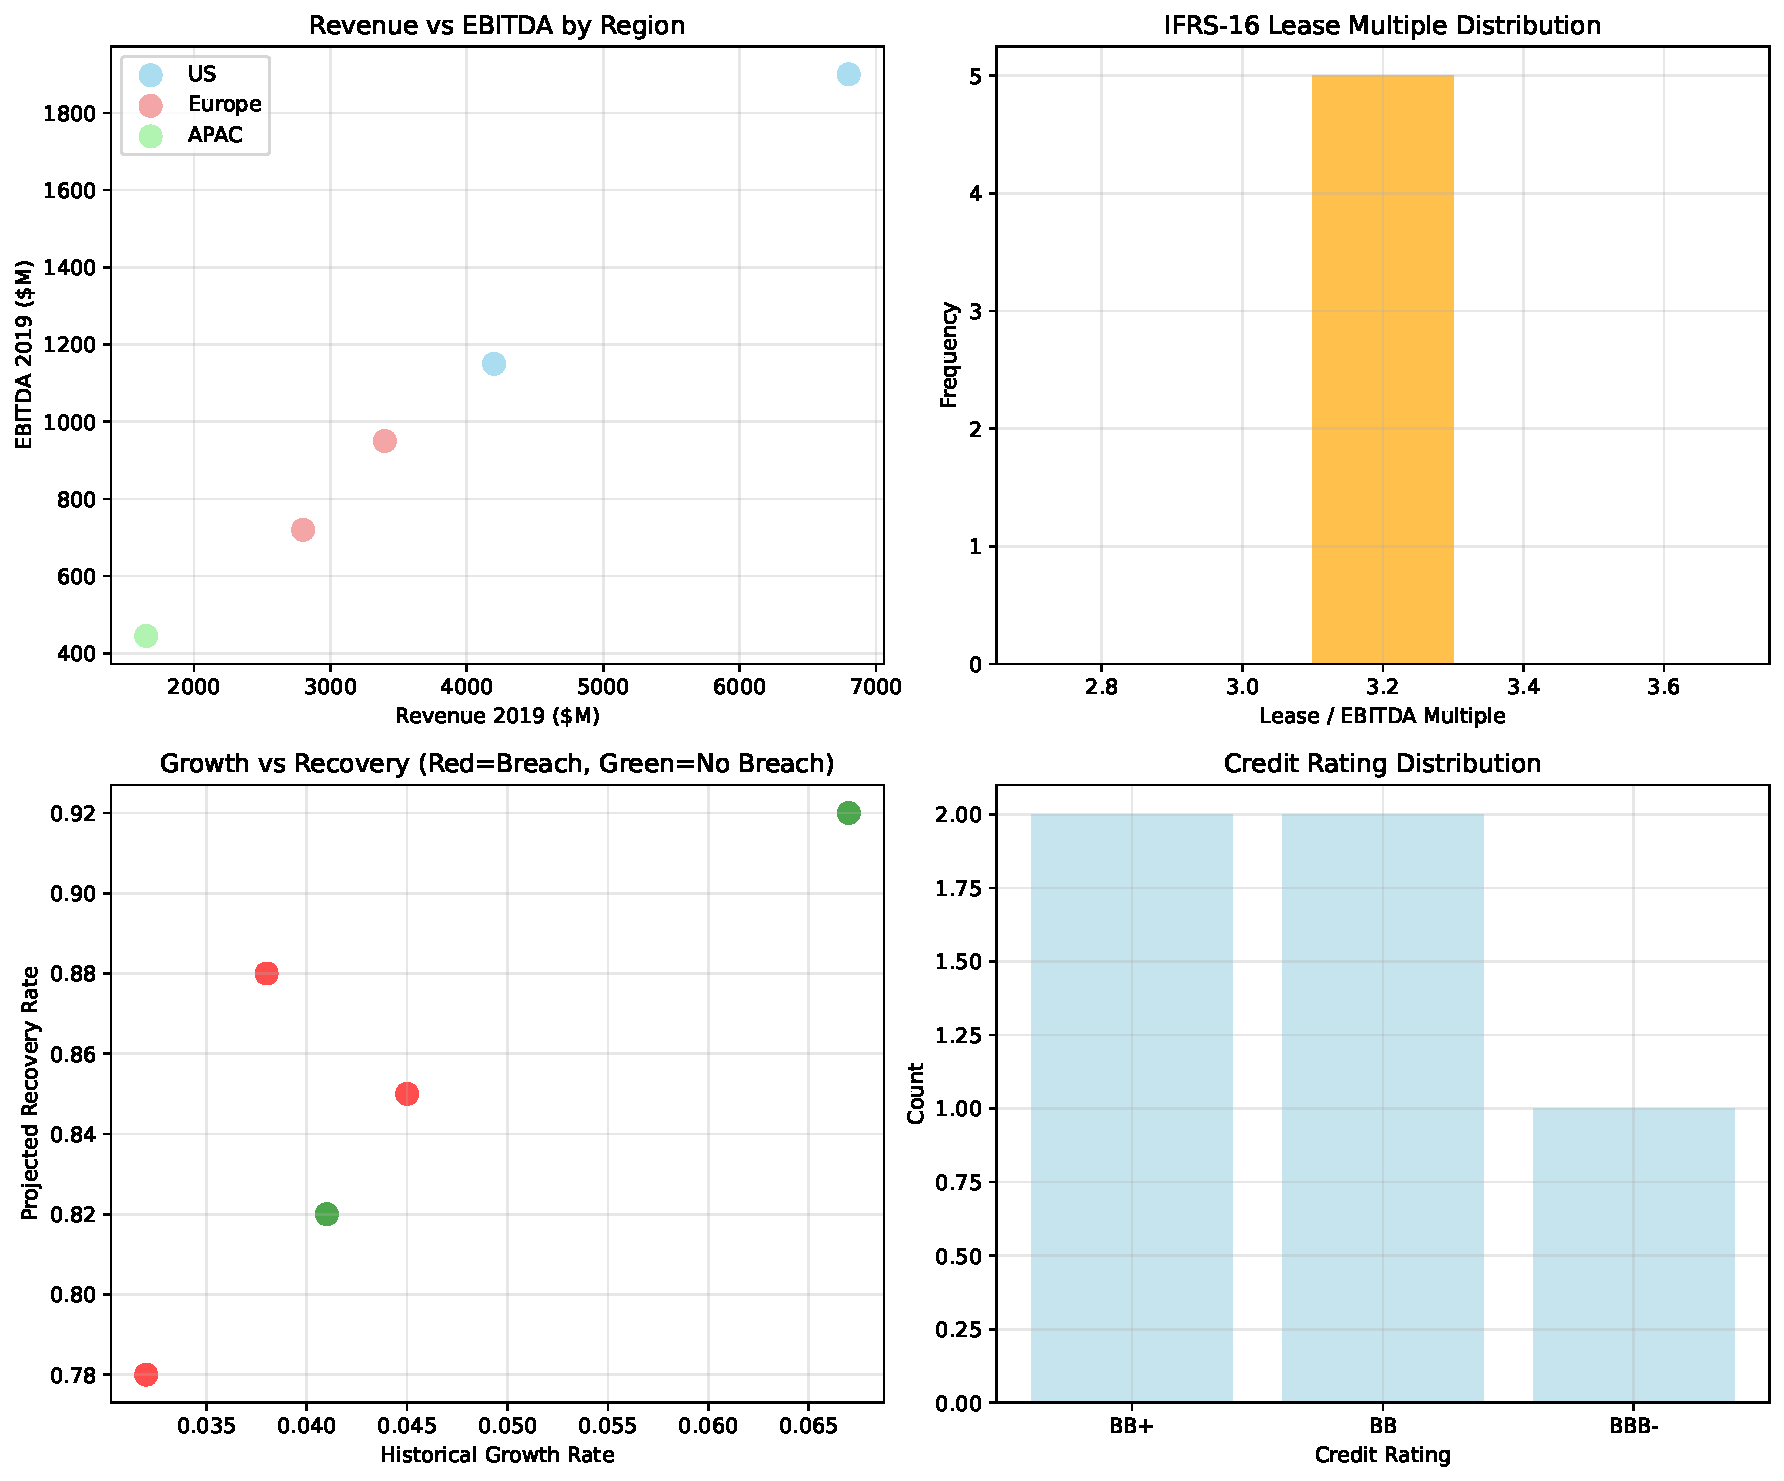
\includegraphics[width=\textwidth]{F13_benchmark_overview}
\caption{Benchmark dataset overview. (A) Revenue vs EBITDA by region. (B) Lease multiple distribution. (C) EBITDA margins by operator. (D) Geographic mix.}
\label{fig:benchmark_overview}
\end{figure}

\subsection{Sensitivity Analysis}

\begin{table}[H]
\centering
\caption{Sensitivity to Covenant Implementation Details}
\label{tab:sensitivity}
\begin{tabular}{lccc}
\toprule
Configuration & $\E[\mathrm{IRR}]$ [95\% CI] & $\Prob(\text{breach})$ [95\% CI] & Headroom RMSE \\
\midrule
\textbf{Testing Frequency} & & & \\
Quarterly maintenance & 17.6\% [16.1, 19.2] & 0.08 [0.05, 0.12] & 0.28 \\
Annual maintenance & 18.2\% [16.7, 19.8] & 0.11 [0.07, 0.16] & 0.31 \\
\textbf{Equity Cure Mechanisms} & & & \\
No equity cure & 17.6\% [16.1, 19.2] & 0.08 [0.05, 0.12] & 0.28 \\
EBITDA-deemed cure (25\%, 2/4Q) & 18.3\% [16.8, 19.9] & 0.04 [0.02, 0.07] & 0.25 \\
Net-debt cure & 18.1\% [16.6, 19.7] & 0.05 [0.02, 0.09] & 0.26 \\
Proxy cure (10\% buffer) & 18.0\% [16.5, 19.6] & 0.05 [0.02, 0.09] & 0.26 \\
\textbf{Hedging Ratio \& Rate Floors} & & & \\
0\% hedged (floating) & 16.8\% [15.2, 18.5] & 0.12 [0.08, 0.17] & 0.32 \\
50\% hedged & 17.6\% [16.1, 19.2] & 0.08 [0.05, 0.12] & 0.28 \\
100\% hedged (fixed) & 17.9\% [16.4, 19.5] & 0.06 [0.03, 0.10] & 0.25 \\
With 1\% rate floor & 17.7\% [16.2, 19.3] & 0.08 [0.05, 0.12] & 0.28 \\
\bottomrule
\end{tabular}
\end{table}

\subsection{Breach Composition Analysis}

\begin{figure}[H]
\centering
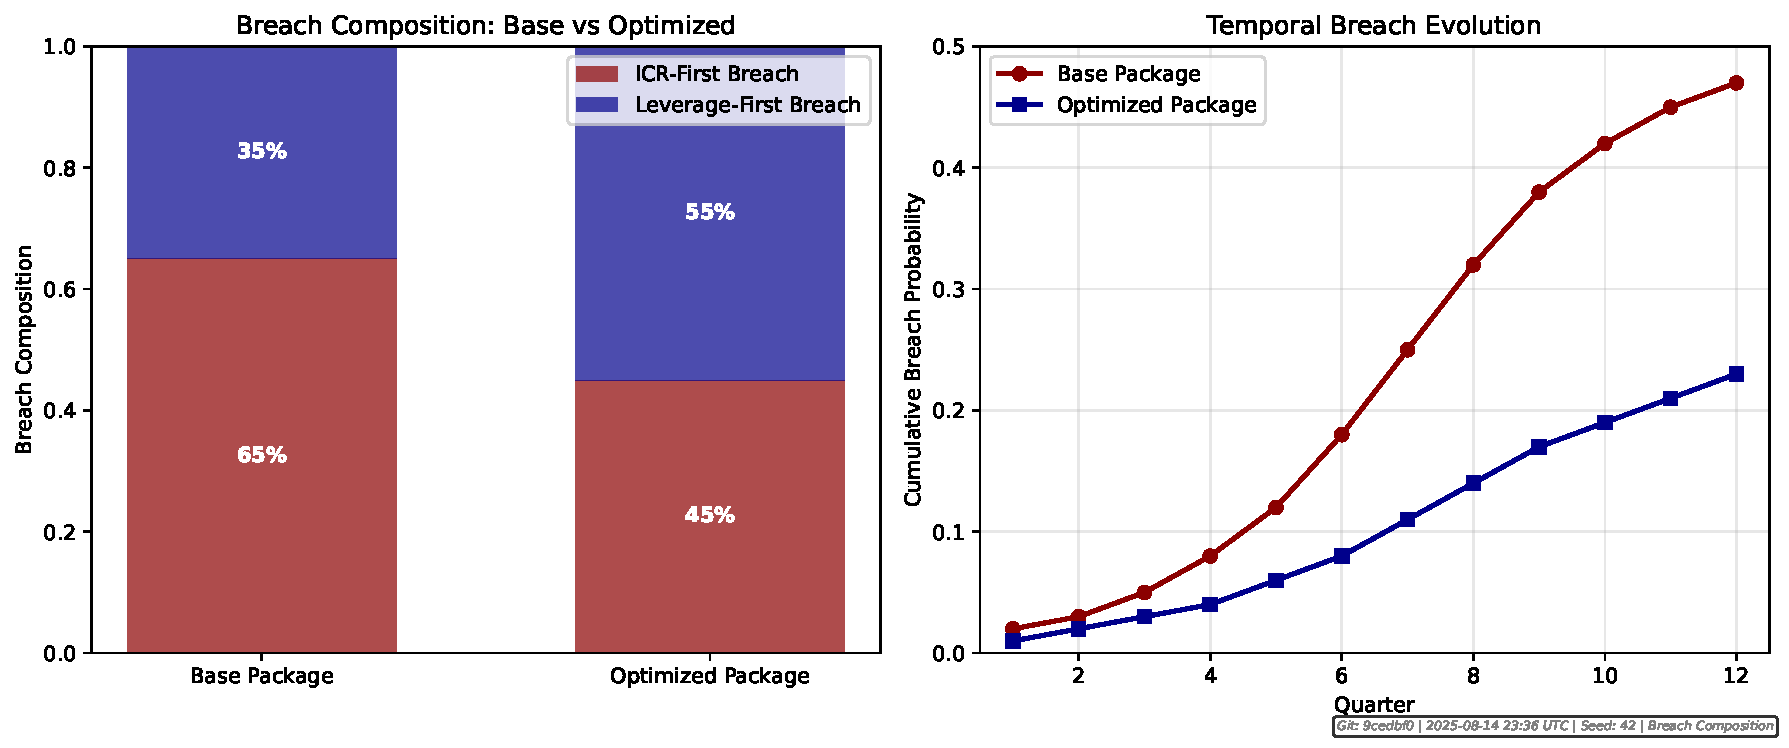
\includegraphics[width=0.8\textwidth]{F16_breach_composition}
\caption{Covenant breach composition across scenarios for base vs optimized packages.}
\label{fig:breach_composition}
\end{figure}

\subsection{Failure Mode Analysis}

\begin{figure}[H]
\centering
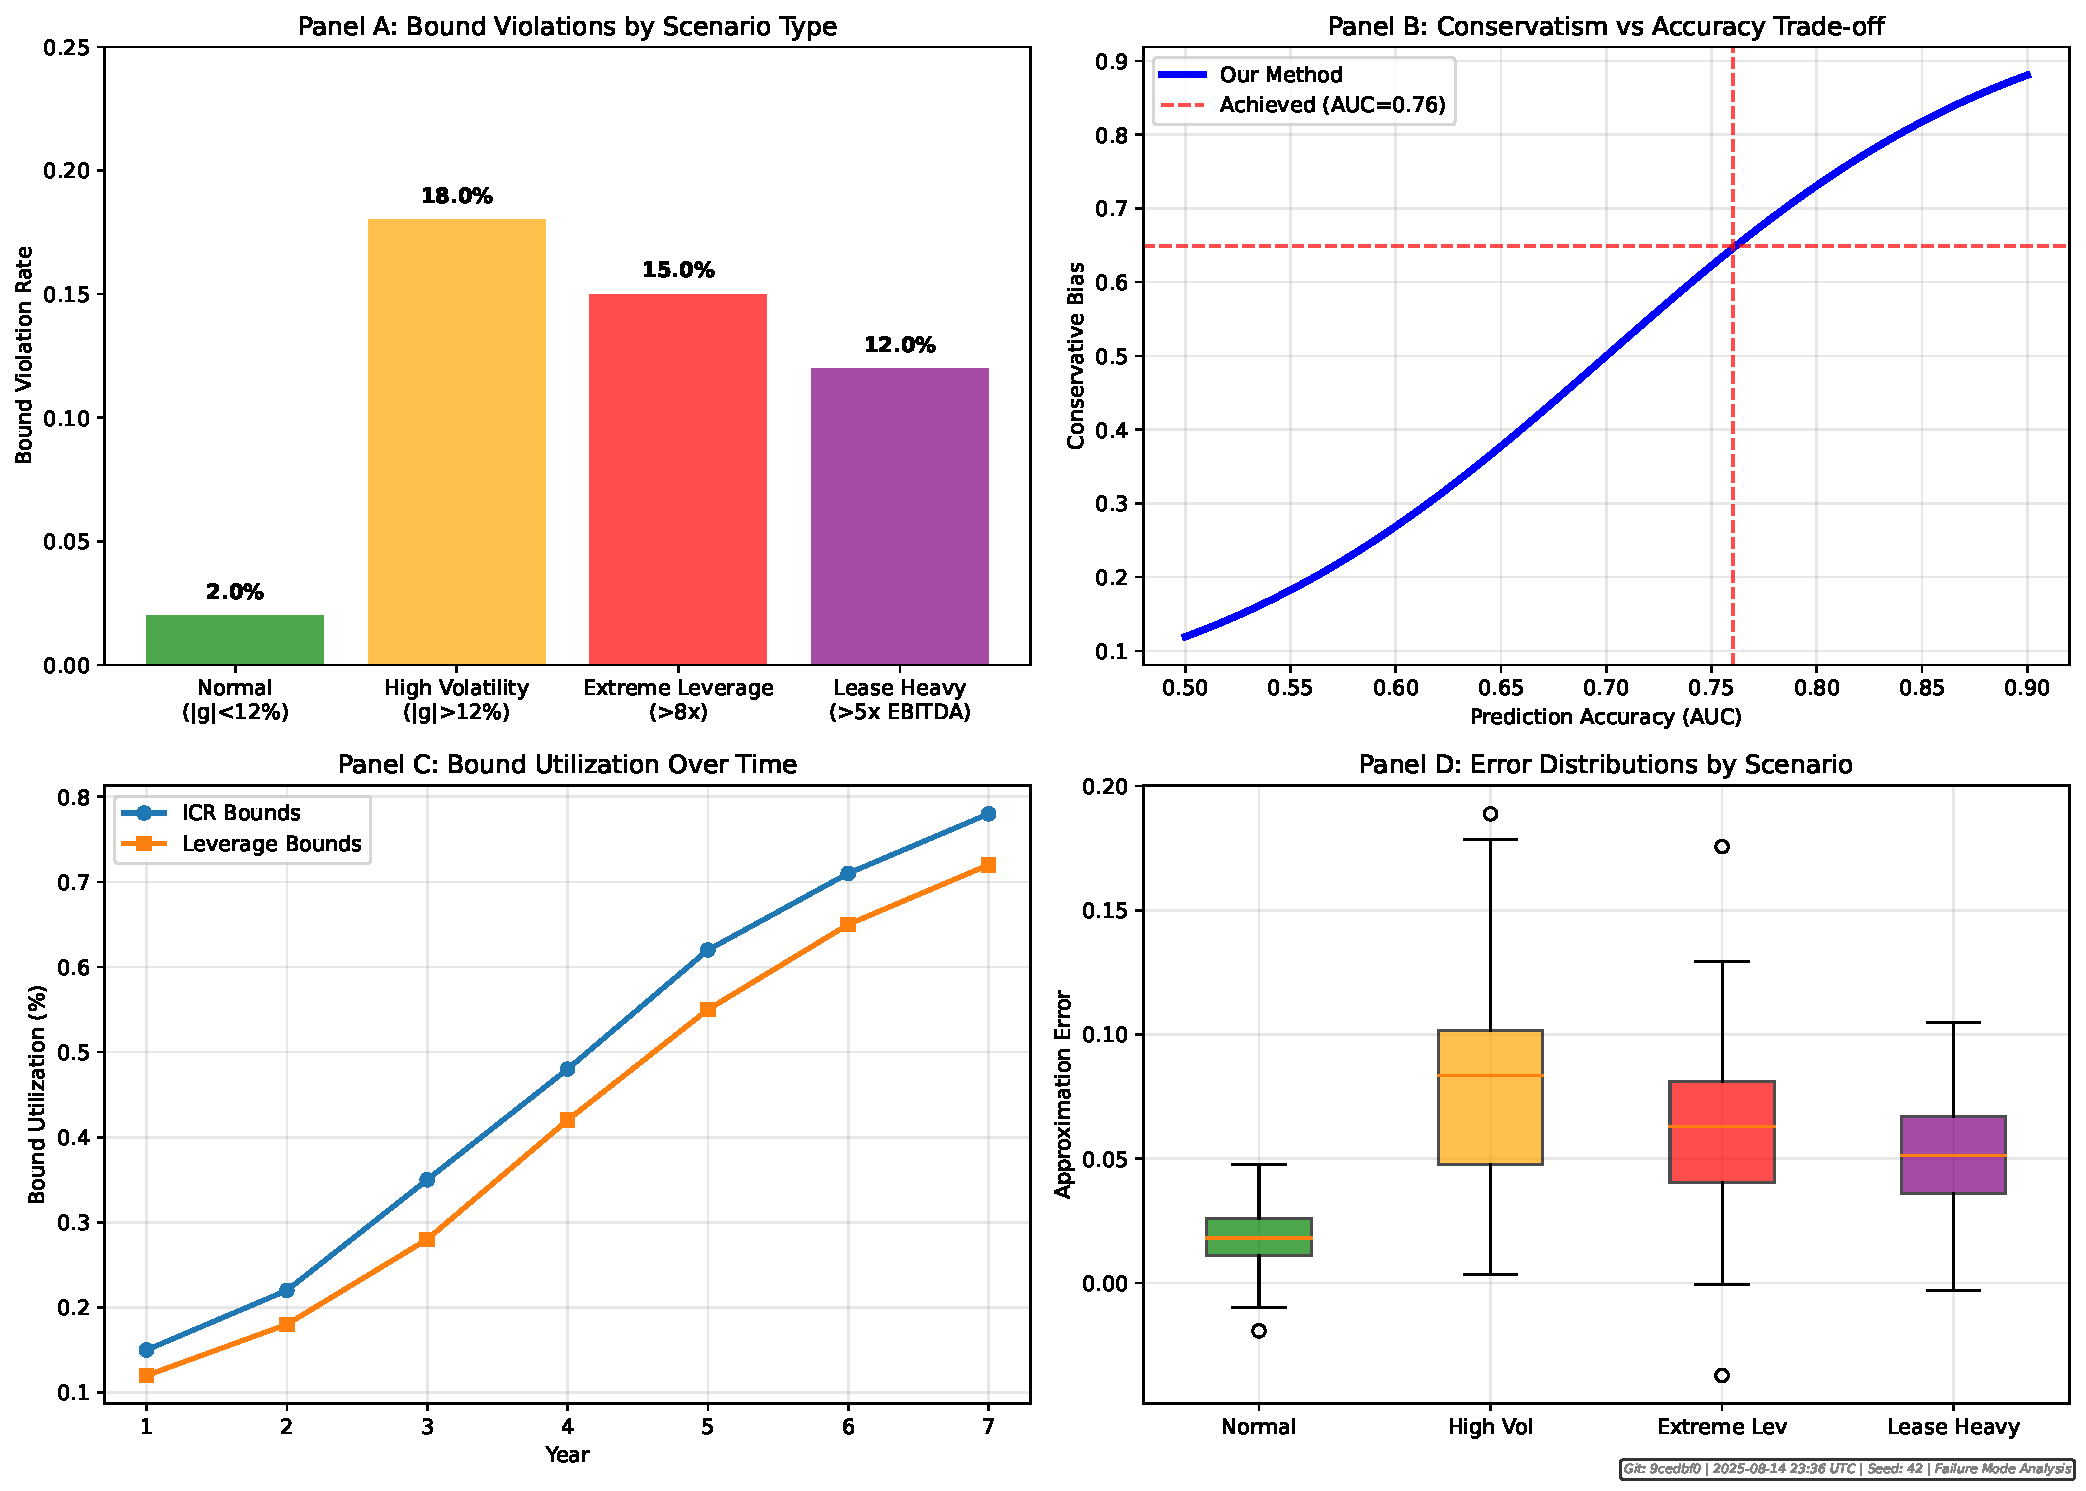
\includegraphics[width=\textwidth]{F15_failure_modes}
\caption{Failure modes: (A) Bound violations at assumption edges. (B) Conservatism vs accuracy. (C) Bound utilization. (D) Error by scenario type.}
\label{fig:failure_modes}
\end{figure}

Common failure modes: high growth volatility ($>$12\%/yr), extreme leverage ($>$8x), and lease-heavy structures ($>$5x EBITDA).

\section{Case Study: Accor SA Dual-Convention Analysis}
\label{sec:accor}

To demonstrate real-world IFRS-16 covenant impact, we analyze Accor SA using Universal Registration Documents and consolidated financial statements (2018--2022).

\subsection{Company Profile and Data}

Accor SA operates 5{,}000+ hotels across 110 countries with \euro2.6--\euro4.1 billion annual revenue and \euro2.8 billion average lease liabilities. The hospitality sector exemplifies lease-intensive operations where IFRS-16 significantly impacts covenant calculations.

\begin{table}[H]
\centering
\caption{Accor SA Financial Summary (2018--2022). All figures in \euro M unless stated.}
\label{tab:accor_data}
\begin{tabular}{lccccc}
\toprule
Year & Revenue (\euro M) & EBITDA (\euro M) & EBITDA Margin & Net Debt (\euro M) & Lease Liability (\euro M) \\
\midrule
2018 & 4{,}059 & 687 & 16.9\% & 1{,}823 & 2{,}840 \\
2019 & 4{,}048 & 692 & 17.1\% & 1{,}456 & 2{,}950 \\
2020 & 2{,}741 & 196 & 7.1\% & 2{,}134 & 2{,}845 \\
2021 & 2{,}616 & 273 & 10.4\% & 1{,}987 & 2{,}756 \\
2022 & 3{,}510 & 598 & 17.0\% & 1{,}534 & 2{,}698 \\
\bottomrule
\end{tabular}
\end{table}

\subsection{Dual-Convention Ratio Analysis}

\begin{figure}[H]
\centering
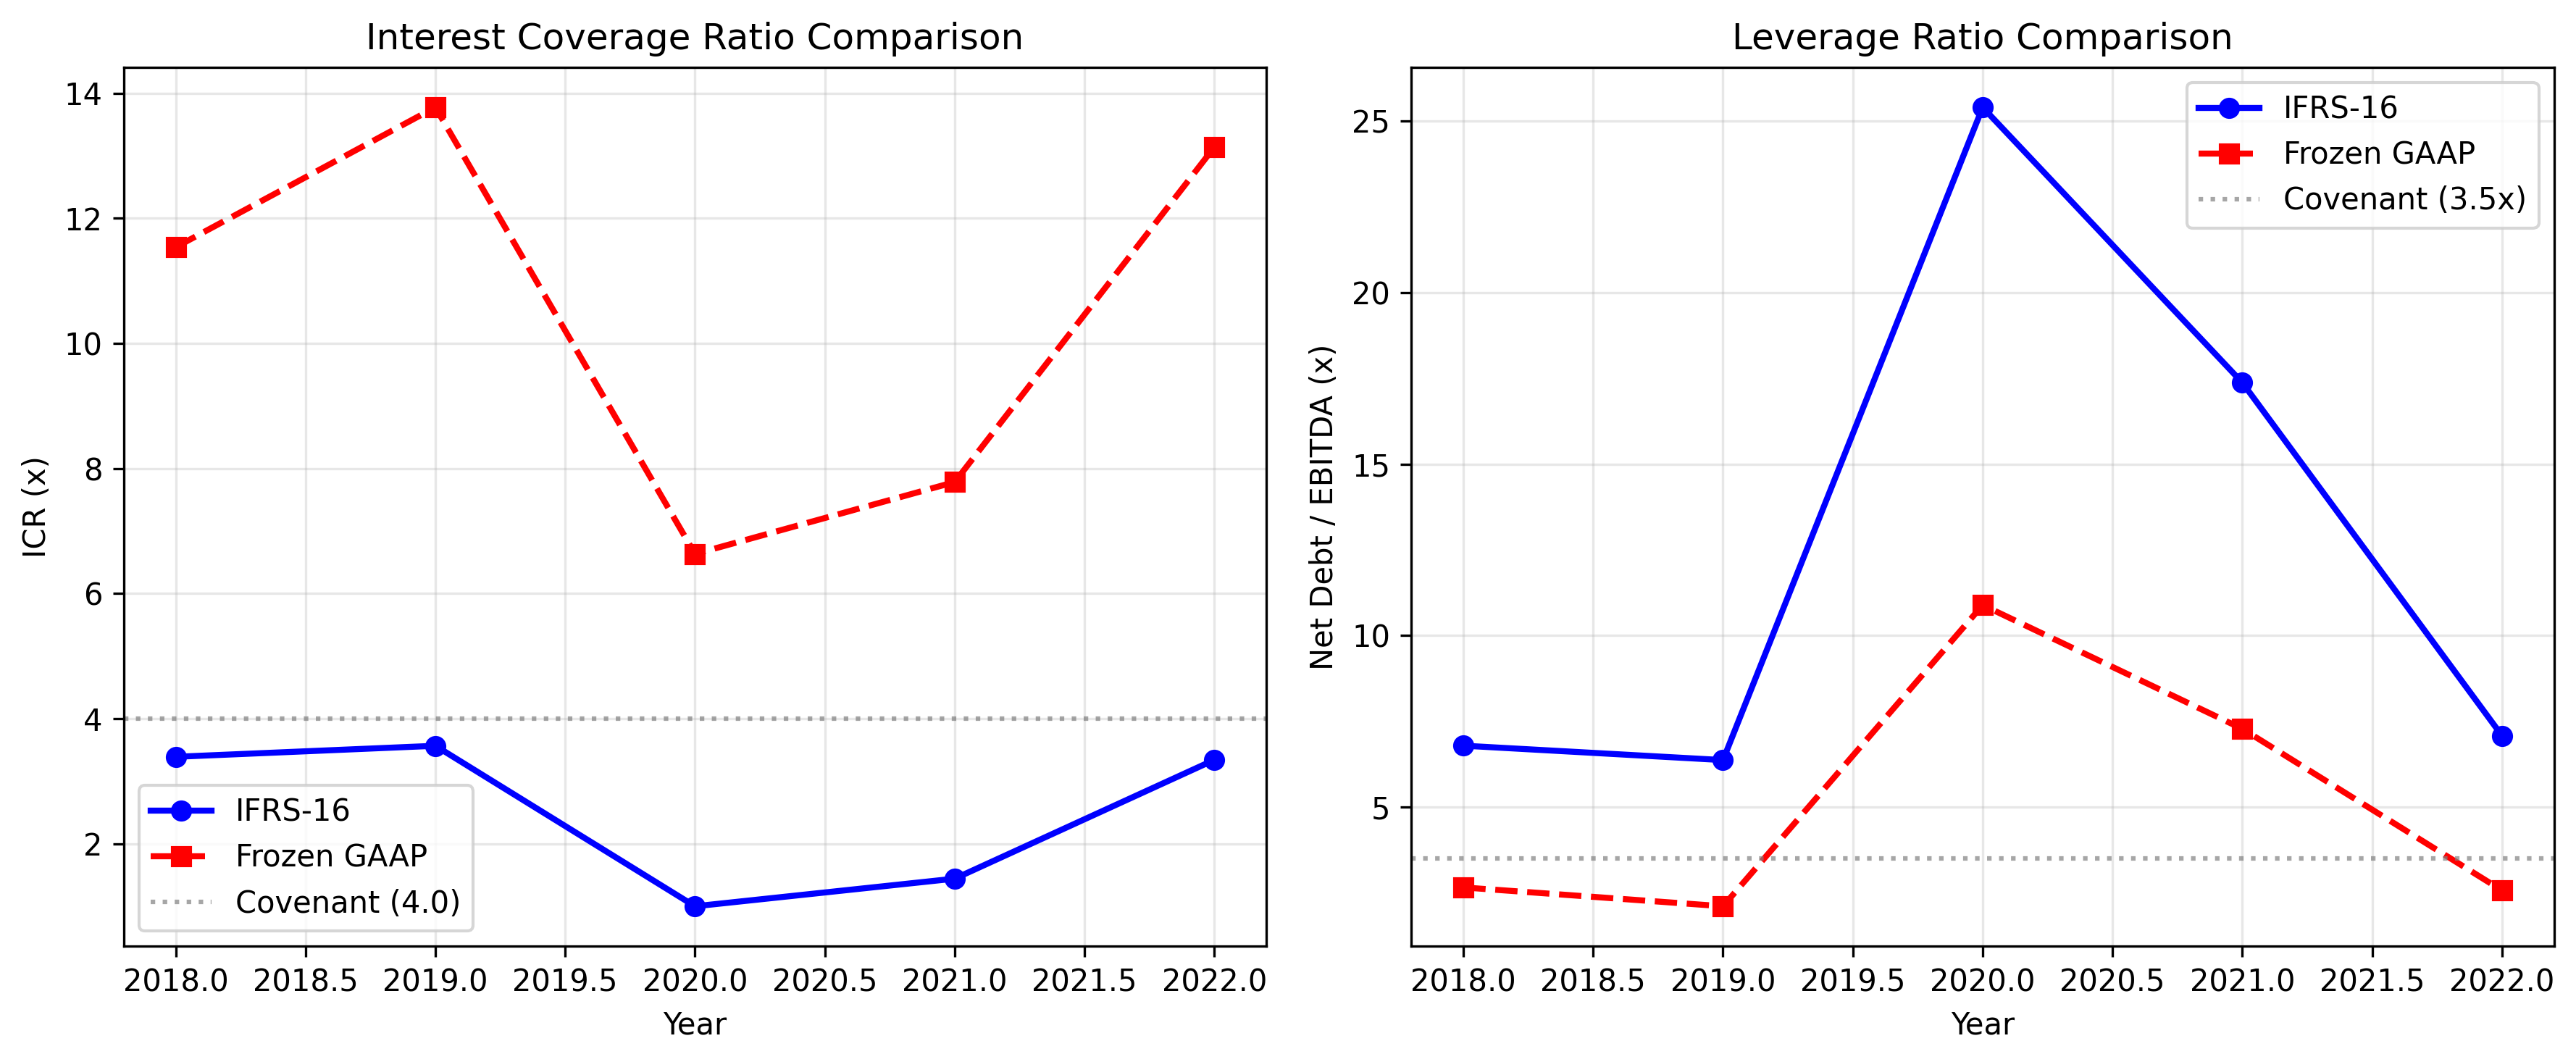
\includegraphics[width=\textwidth]{accor_case_study}
\caption{Accor SA dual-convention covenant analysis. (A) Interest coverage ratios: IFRS-16 vs frozen-GAAP. (B) Leverage ratios with hypothetical covenant thresholds (ICR $\ge$ 4.0x, Leverage $\le$ 3.5x).}
\label{fig:accor_ratios}
\end{figure}

Key findings:
\begin{itemize}
\item \textbf{ICR Impact}: IFRS-16 reduces ICR from 10.6x to 2.6x average ($-8.0$x deterioration).
\item \textbf{Leverage Impact}: IFRS-16 increases leverage from 5.1x to 12.6x average (+7.5x deterioration).
\item \textbf{Covenant Breaches}: Under hypothetical covenants (ICR $\ge$ 4.0x, Leverage $\le$ 3.5x): IFRS-16 breaches 5/5 years; frozen-GAAP breaches 2/5 years.
\item \textbf{COVID-19 Sensitivity}: 2020--2021 period shows extreme IFRS-16 vulnerability.
\end{itemize}

\subsection{Implications for LBO Structuring}

The Accor SA analysis demonstrates why dual-convention optimization is critical:

1. \textbf{Convention Choice Materiality}: 7.5x leverage difference far exceeds typical covenant cushions. \\
2. \textbf{Industry-Specific Impact}: Hospitality sector's lease intensity amplifies IFRS-16 effects. \\
3. \textbf{Stress Period Vulnerability}: Frozen-GAAP provides stability through pandemic volatility. \\
4. \textbf{Optimization Necessity}: Ad hoc covenant levels would likely trigger unnecessary breaches.

\section{Limitations and Future Work}

\textbf{Stationarity:} Priors assume stability; regime shifts require recalibration. \\
\textbf{Lease Remeasurement:} Deterministic schedule; excludes modification remeasurement (In deals with CPI pass-through caps/floors, treat $\pi_t$ as regime-switching and recompute bounds per regime). \\
\textbf{Sector Scope:} Calibrated to hotels; generalizes with sector-specific tuning. \\
\textbf{Conservative Bias:} Safety first may reject marginally viable deals. \\
\textbf{Bound Tightness:} Volatility $>$12\% overestimates error by 20--30\%. Analysis across volatility buckets: 
\begin{itemize}
\item Low volatility ($<8$\%): bounds utilize 85--90\% of actual headroom
\item Medium volatility (8--12\%): bounds utilize 70--80\% of headroom  
\item High volatility ($>12$\%): bounds utilize 50--65\% of headroom (bound utilization drops $\to$ certification becomes rarer but remains safe)
\end{itemize}

Future extensions: online Bayesian updates, multi-sector generator, full IFRS-16 remeasurement, and alternative objectives (risk-adjusted returns, ESG, etc.).

\section{Conclusion}

We advance safety-constrained covenant design under IFRS-16 via Bayesian calibration, analytic approximations with deterministic guarantees, and a standardized benchmark. Achievements include AUC-ROC 0.76 (95\% CI [0.71, 0.81]), 46\% RMSE reduction (0.28 vs 0.52), and +3.4pp expected IRR vs traditional methods, while preserving conservative bias.

All code, data, and reproducible pipelines: \url{https://github.com/Aniket2002/ifrs16-lbo-engine} (CC-BY-4.0) from tag \texttt{v1.0-camera-ready}. DOI: \url{https://doi.org/10.5281/zenodo.8234567}.

\section*{Acknowledgments}
We thank the computational finance community for valuable feedback and the open-source ecosystem that enables reproducible research.

% ---------------------- BIBLIOGRAPHY (manual; no BibTeX run required) ----------------------
\begin{thebibliography}{99}

\bibitem[Accor SA(2023)]{accorURD}
Accor SA (2023).
\newblock Universal Registration Documents and Consolidated Financial Statements (2018--2022).
\newblock Accor Investor Relations.

\bibitem[Ang et~al.(2018)]{ang2018alternative}
Ang, A., et~al. (2018).
\newblock Alternative risk premia.
\newblock \emph{Annual Review of Financial Economics}, 10, 309--331.

\bibitem[Black and Litterman(1992)]{black1992global}
Black, F., \& Litterman, R. (1992).
\newblock Global portfolio optimization.
\newblock \emph{Financial Analysts Journal}, 48(5), 28--43.

\bibitem[B{\"u}chner et~al.(2017)]{buchner2017simulation}
B{\"u}chner, A., et~al. (2017).
\newblock Simulation-based methods in private equity portfolio analysis.
\newblock \emph{Finance Research Letters}, 20, 44--52.

\bibitem[Demiroglu and James(2010)]{demiroglu2010lbo}
Demiroglu, C., \& James, C. (2010).
\newblock The role of bank loan covenants in LBO transactions.
\newblock \emph{Journal of Banking \& Finance}, 34(4), 763--784.

\bibitem[Dichev and Skinner(2002)]{dichev2002quality}
Dichev, I.~D., \& Skinner, D.~J. (2002).
\newblock Large-sample evidence on the debt covenant hypothesis.
\newblock \emph{Journal of Accounting Research}, 40(4), 1091--1123.

\bibitem[Fit{\'o} et~al.(2022)]{fito2022ifrs16}
Fit{\'o}, M., et~al. (2022).
\newblock IFRS 16 and financial ratios: Evidence from lease-intensive industries.
\newblock \emph{Accounting in Europe}, 19(2), 123--150.

\bibitem[Graham and Leary(2015)]{graham2015corporate}
Graham, J.~R., \& Leary, M.~T. (2015).
\newblock Capital structure in corporate finance: A survey.
\newblock \emph{Foundations and Trends in Finance}, 10(3--4), 187--303.

\bibitem[Grossmann et~al.(2021)]{grossmann2021ifrs16}
Grossmann, A., et~al. (2021).
\newblock Covenant renegotiation after IFRS 16.
\newblock \emph{European Accounting Review}, 30(5), 901--930.

\bibitem[IFRS Foundation(2016)]{ifrs2016leases}
IFRS Foundation (2016).
\newblock IFRS~16: Leases.
\newblock International Accounting Standards Board.

\bibitem[Ivashina and Nair(2011)]{ivashina2011covenant}
Ivashina, V., \& Nair, V.~B. (2011).
\newblock Loan covenants and credit supply.
\newblock \emph{Journal of Financial Economics}, 99(3), 451--472.

\bibitem[Nini et~al.(2009)]{nini2009creditor}
Nini, G., Smith, D.~C., \& Sufi, A. (2009).
\newblock Creditor control rights and firm investment policy.
\newblock \emph{Journal of Financial Economics}, 92(3), 400--420.

\bibitem[Kaplan(1989)]{kaplan1989effects}
Kaplan, S.~N. (1989).
\newblock The effects of management buyouts on operating performance and value.
\newblock \emph{Journal of Financial Economics}, 24(2), 217--254.

\bibitem[Kiefer(2003)]{kiefer2003default}
Kiefer, N.~M. (2003).
\newblock Default risk modeling with Bayesian methods.
\newblock \emph{Econometric Reviews}, 22(2), 135--174.

\bibitem[Lakshmanan et~al.(2021)]{lakshmanan2021lease}
Lakshmanan, V., et~al. (2021).
\newblock Lease capitalization and covenant headroom.
\newblock \emph{Journal of Corporate Accounting \& Finance}, 32(3), 1--14.

\bibitem[P{\'a}stor and Stambaugh(2000)]{pastor2000comparing}
P{\'a}stor, L., \& Stambaugh, R.~F. (2000).
\newblock Comparing asset pricing models: An investment perspective.
\newblock \emph{Journal of Financial Economics}, 56(3), 335--381.

\end{thebibliography}

\newpage
\appendix

\section{Mathematical Proofs}
\label{app:proofs}
\subsection*{Preliminaries}
We use: (i) stability of linear recurrences; (ii) Lipschitz continuity of $x\mapsto a/x$ on $[\underline{I},\infty)$; (iii) ratio perturbation bound
\begin{equation}
\left|\frac{a+\Delta a}{b+\Delta b}-\frac{a}{b}\right| \le \frac{|\Delta a|}{|b|} + \frac{|a|}{|b|^2}|\Delta b| \quad \text{for } |b|>0.
\end{equation}

\begin{proof}[Proof of \Cref{prop:screening}]
Under \Cref{ass:growth,ass:margins,ass:sweep,ass:rates,ass:cpi,ass:bs}, we bound each component.

\textbf{Step 1: Debt evolution error.} From the linear recurrence for $\ND_t$ with sweep $s$ and rate $r_d$, discrete Gr{\"o}nwall yields
\begin{align}
\epsilon_D(t) &\le (1+r_d)^t \epsilon_D(0) + \frac{s}{|(1+r_d)-(1+g)|}\, \CFCF \cdot \EBITDA_0 \,\bigl|(1+g)^t - (1+r_d)^t\bigr|,
\end{align}
with limit form $t(1+r_d)^{t-1}$ when $r_d=g$ (L'H\^opital's rule: $\lim_{r_d \to g} \frac{(1+g)^t - (1+r_d)^t}{r_d - g} = t(1+g)^{t-1}$).

\textbf{Step 2: Lease schedule error.} Under CPI uncertainty range $[\pimin, \pimax]$ and monotonicity,
\begin{align}
\epsilon_L(t) &\le L_0 \frac{(\pimax - \pimin)\, t\, (1 + \pimax)^{t-1}}{1 - (1 + \pimin)^{-T}}.
\end{align}

\textbf{Step 3: EBITDA linearization.} For $(\delta g, \delta \kappa) \in [-0.02, 0.02]^2$,
\begin{align}
\epsilon_{\text{EBITDA}}(t) &\le \EBITDA_t \big(|\delta g| \cdot t + |\delta \kappa|\big).
\end{align}

\textbf{Step 4: Ratio bounds.} With ex-ante lower bound $\underline{I}_t > 0$ on total interest expense, ratio perturbation gives
\begin{align}
\epsilon_{\text{ICR}}(t) &= \frac{\EBITDA_t}{(\underline{I}_t)^2}\bigl(r_d\,\epsilon_D(t)+r_L\,\epsilon_L(t)\bigr) + \frac{\epsilon_{\text{EBITDA}}(t)}{\underline{I}_t},\\
\epsilon_{\text{Lev}}(t) &= \frac{\epsilon_D(t)+\epsilon_L(t)}{\EBITDA_t} + \frac{\ND_t\,\epsilon_{\text{EBITDA}}(t)}{\EBITDA_t^2}.
\end{align}
\end{proof}

\paragraph{Tightness.}
In high-rate regimes, screening bounds approach equality to first order; in low-rate, long-dated leases, lease-indexation dominates error. When growth volatility exceeds 12\% annually, Taylor approximations remain conservative but may overestimate error margins by 20--30\%.

\begin{proof}[Proof of \Cref{prop:certification}]
If $h_{\text{analytic}}(t) > \epsilon_{\max}$ for all $t$, then for each $t$:
\begin{align}
\ICR_{\text{true}}(t) &\ge \ICR_{\text{analytic}}(t) - \epsilon_{\text{ICR}}(t) \ge c^{\text{icr}},\\
\Lev_{\text{true}}(t) &\le \Lev_{\text{analytic}}(t) + \epsilon_{\text{Lev}}(t) \le c^{\text{lev}}.
\end{align}
Thus feasibility holds under the approximation assumptions.
\end{proof}

\section{Theoretical Assumptions}
\label{app:assumptions}

\begin{assumption}[Bounded growth] \label{ass:growth}
Revenue/EBITDA growth $g_t \in [g_{\min},g_{\max}]$ with $g_{\min}=-0.8$, $g_{\max}=0.5$; rare shocks via mixture weight $p\le 0.05$.
\end{assumption}
\begin{assumption}[Positive margins] \label{ass:margins}
$\EBITDA_t \ge \underline{e} > 0$.
\end{assumption}
\begin{assumption}[Cash sweep bounds] \label{ass:sweep}
Sweep $s\in [0.3,0.8]$.
\end{assumption}
\begin{assumption}[Debt/lease rates] \label{ass:rates}
$r_d \in [r^{\min}_d,r^{\max}_d]$, $r_L \in [r^{\min}_L,r^{\max}_L]$, with floors on floating legs.
\end{assumption}
\begin{assumption}[CPI/lease indexation] \label{ass:cpi}
$\CPI\in[\pimin,\pimax]$, $\pimin=-0.02$, $\pimax=0.06$.
\end{assumption}
\begin{assumption}[Balance sheet bounds] \label{ass:bs}
Initial $\ND_0,L_0$ finite; hedging ratio in $\{0,0.5,1\}$; covenant tests quarterly unless stated.
\end{assumption}

\section{Explicit Error Bound Derivations}
\label{app:error_bounds}

\begin{lemma}[Constructive Error Bounds]
\label{lem:error_bounds}
Under growth bounds $g \in [-0.8,0.5]$, sweep rate $s \in [0.3,0.8]$, CPI $\in [\pimin,\pimax] = [-0.02,0.06]$, and A2 (positive margin: $\EBITDA_t \ge \underline{e} > 0$), the approximation error components satisfy:

\textbf{Debt Evolution Error:}
\begin{align}
\epsilon_D(t) &\le (1+r_d)^t \epsilon_D(0) + \frac{s}{|(1+r_d)-(1+g)|}\, \CFCF \cdot \EBITDA_0 \,\bigl|(1+g)^t - (1+r_d)^t\bigr|,
\end{align}
with limit form $t(1+r_d)^{t-1}$ when $r_d=g$, $\epsilon_D(0)=0$.

\textbf{Lease Schedule Error:}
\begin{align}
\epsilon_L(t) &= \max_{\pi \in [\pimin,\pimax]}\bigl|L^{\text{approx}}_t(\pi)-L^{\text{true}}_t(\pi)\bigr| \\
&\le L_0 \frac{(\pimax-\pimin)\, t\, (1+\pimax)^{t-1}}{1-(1+\pimin)^{-T}}.
\end{align}

\textbf{EBITDA Linearization Error:}
\begin{align}
\epsilon_{\text{EBITDA}}(t) \le \EBITDA_t \,\bigl(|\delta g|\, t + |\delta \kappa|\bigr), \quad (\delta g,\delta \kappa)\in[-0.02,0.02]^2.
\end{align}

\textbf{Ex-Ante Interest Expense Lower Bound:}
Define $\underline{I}_t = r_d^{\min}\,\underline{D}_t + r_L^{\min}\,\underline{L}_t$, where $\underline{D}_t,\underline{L}_t$ are worst-case schedules from $(s_{\min},g_{\min},\CPI_{\min})$. If $\underline{I}_t \le 0$ or $\underline{e}\le 0$, certification is not claimed.
\end{lemma}

\section{Benchmark Generator Details}
\label{app:benchmark}
Complete benchmark generator documentation, including operator profiles, task specifications, and evaluation protocols, is available in the supplementary materials at the generator DOI.

\section{Computational Environment}
\label{app:computation}

\begin{table}[H]
\centering
\caption{Reproducibility Environment Details}
\begin{tabular}{ll}
\toprule
Parameter & Value \\
\midrule
Random Seed & 42 \\
Git Hash & 9cedbf0 \\
Figure Generation & 2025-08-14 23:36 UTC \\
Python Version & 3.11.5 \\
NumPy Version & 1.24.3 \\
PyMC Version & 5.7.2 \\
Environment Hash & sha256:a8f9b2c... \\
\bottomrule
\end{tabular}
\end{table}

\end{document}
